\documentclass[11pt,a4paper]{article}

\usepackage[utf8]{inputenc}
\usepackage[T1]{fontenc}
\usepackage{lmodern}
\usepackage{geometry}
\usepackage{graphicx}
\usepackage{booktabs}
\usepackage{array}
\usepackage{multirow}
\usepackage{float}
\usepackage{subcaption}
\usepackage{xcolor}
\usepackage{amsmath}
\usepackage{amssymb}
\usepackage{hyperref}
\usepackage{enumitem}
\usepackage{listings}
\usepackage{longtable}
\usepackage{caption}
\usepackage{microtype}

\geometry{margin=2.35cm}
\hypersetup{
    colorlinks=true,
    linkcolor=blue!50!black,
    citecolor=blue!50!black,
    urlcolor=blue!50!black
}

\definecolor{lightgray}{gray}{0.96}
\definecolor{darkblue}{RGB}{25,55,115}
\definecolor{darkgreen}{RGB}{32,105,66}
\definecolor{darkred}{RGB}{150,45,45}

\lstdefinestyle{pythonstyle}{
    language=Python,
    basicstyle=\ttfamily\small,
    backgroundcolor=\color{lightgray},
    frame=single,
    rulecolor=\color{gray!50},
    breaklines=true,
    showstringspaces=false,
    keywordstyle=\color{blue!70!black},
    commentstyle=\color{green!45!black},
    stringstyle=\color{red!60!black}
}

\newcommand{\metric}[1]{\textbf{#1}}
\newcommand{\code}[1]{\texttt{#1}}

\title{\textbf{Multivariate ECG Classification with Deep Learning}\\
\large From a MIT-BIH 1D-CNN Baseline to a PTB-XL Shared-Loss Fusion Model}
\author{Antoine Metz}
\date{May 2026}

\begin{document}

\maketitle

\begin{abstract}
This project studies deep learning for electrocardiogram (ECG) classification. The work first implements a baseline on the MIT-BIH Arrhythmia Database using raw ECG records, heartbeat extraction, and a 1D convolutional neural network. After feedback, the project is extended to PTB-XL, where the task becomes a multivariate and multi-label ECG classification problem. The PTB-XL model uses 12-lead ECG signals as temporal channels and static clinical metadata as additional contextual variables. The final architecture is an end-to-end shared-loss fusion model: a 1D-CNN extracts ECG features, a small MLP extracts metadata features, both representations are concatenated, and a final classifier predicts the five PTB-XL diagnostic superclasses. The project compares ECG-only, metadata-only, soft-voting and feature-level fusion strategies. The best fusion model reaches a test macro-F1 of 0.7108 and a micro-F1 of 0.7536, slightly outperforming the ECG-only baseline and the soft-voting ensemble. The results show that ECG morphology remains the dominant source of information, while metadata provides a modest but useful complementary clinical context.
\end{abstract}

\tableofcontents
\newpage

\section{Introduction}

Electrocardiography is one of the most widely used non-invasive tools for assessing cardiac activity. A standard ECG records the electrical activity of the heart over time and can reveal rhythm abnormalities, conduction disturbances, myocardial infarction patterns, hypertrophy, and repolarization changes. Manual interpretation by experts remains the clinical reference, but automated ECG classification is useful for screening, decision support and large-scale processing of medical signals.

The objective of this project is to build a deep learning pipeline for ECG classification. The project started with a simpler heartbeat-level classification task on the MIT-BIH Arrhythmia Database. This first baseline was useful to validate the basic workflow: loading raw ECG recordings, extracting heartbeat windows, training a 1D-CNN, and computing classification metrics. However, this first task was limited because it used a single ECG channel and classified isolated beats.

Following feedback, the project was extended to PTB-XL, a larger 12-lead ECG dataset with clinical metadata and standardized diagnostic annotations \cite{wagner2020ptbxl}. This changes the problem formulation: instead of classifying one isolated heartbeat, we classify a full 10-second ECG recording with multiple leads and possible multiple diagnostic labels. The new task is therefore a multivariate, multi-label ECG classification problem.

This report presents the full progression of the project. It explains the MIT-BIH baseline, the transition to PTB-XL, the multivariate fusion architecture, the implementation versions, the experimental results, and the final comparison between ECG-only, metadata-only, soft-voting and shared-loss fusion models.

\section{Motivation and Related Work}

Deep learning is well suited for ECG analysis because ECGs are temporal signals with local morphological patterns. A 1D convolutional neural network can learn temporal features such as QRS morphology, ST-segment deviations, rhythm-related changes, and lead-dependent patterns. The use of multiple leads is important because each ECG lead observes the heart's electrical activity from a different spatial viewpoint.

Recent work on PTB-XL shows that strong results can be obtained with relatively simple architectures when the data preparation and training strategy are carefully designed. In particular, Mehdi and Drigh \cite{mehdi2026ptbxl} report competitive performance on PTB-XL using a data-centric CNN-VAE approach, emphasizing preprocessing, class balancing and model simplicity over architectural complexity. Their reported metrics include a weighted F1-score around 0.745 and an AUC around 0.896 across the five diagnostic superclasses. Their architecture is not the same as ours, but their work was used as a reference point for expected performance ranges and for the idea that class imbalance and preprocessing matter strongly in PTB-XL.

The present project does not attempt to reproduce that CNN-VAE architecture. Instead, it focuses on a multimodal fusion question: does static clinical metadata improve a 12-lead ECG classifier, and is it better to fuse metadata at the feature level through a shared-loss model or at the prediction level through soft voting?

\section{Datasets and Problem Formulation}

\subsection{MIT-BIH Baseline Dataset}

The first part used the MIT-BIH Arrhythmia Database, a standard benchmark for arrhythmia analysis \cite{moody2001mitdb,goldberger2000physiobank}. The raw ECG records and expert annotations were loaded using WFDB. Each expert annotation marks the temporal location and type of a heartbeat. Around each annotated beat, a fixed-size window of 187 samples was extracted, normalized independently, and mapped into five heartbeat categories: Normal, Supraventricular, Ventricular, Fusion and Unknown.

The MIT-BIH problem is a standard multi-class classification task:
\[
    x_i \in \mathbb{R}^{1 \times 187}, \qquad y_i \in \{0,1,2,3,4\}.
\]
The model predicts exactly one class per heartbeat, so CrossEntropyLoss is appropriate.

\subsection{PTB-XL Multivariate Dataset}

The main part uses PTB-XL, a large public dataset of 12-lead ECG recordings \cite{wagner2020ptbxl}. Each recording is a 10-second ECG sampled at 100 Hz in our experiments, giving 1000 time samples per lead. The ECG input is represented as:
\[
    X_{ECG} \in \mathbb{R}^{12 \times 1000}.
\]
The 12 channels correspond to the standard ECG leads:
\[
    I, II, III, aVR, aVL, aVF, V1, V2, V3, V4, V5, V6.
\]

The task predicts five diagnostic superclasses:
\[
    \{\text{NORM}, \text{MI}, \text{STTC}, \text{CD}, \text{HYP}\}.
\]
Unlike the MIT-BIH baseline, PTB-XL is naturally multi-label. One ECG can have more than one diagnosis. Therefore, the target is a binary vector:
\[
    y_i \in \{0,1\}^{5}.
\]
The model outputs five logits, one per diagnostic superclass. Each label is treated as a separate binary decision, so the loss is BCEWithLogitsLoss rather than CrossEntropyLoss.

\subsection{Metadata Selection}

The PTB-XL metadata table contains 28 columns, but not all of them are valid clinical input features. Some columns are identifiers, file paths, split information, reports, or diagnostic codes. Using diagnostic code columns directly would introduce label leakage because those codes are used to construct the targets.

For this reason, only four simple static metadata variables were retained:
\[
    \text{age}, \text{sex}, \text{height}, \text{weight}.
\]
These variables are not temporal signals, so they should not be treated as additional CNN channels. Instead, they are processed by a separate MLP branch.

\section{Methodology}

\subsection{MIT-BIH 1D-CNN Baseline}

The MIT-BIH baseline uses a single-channel 1D-CNN. Its input shape is:
\[
    (\text{batch size}, 1, 187).
\]
The model contains several Conv1D blocks followed by pooling and fully connected layers. This baseline was mainly used to validate the ECG preprocessing and training pipeline before moving to PTB-XL.

\subsection{PTB-XL Shared-Loss Fusion Architecture}

The main PTB-XL architecture is a feature-level fusion model. It has two branches:
\begin{itemize}[noitemsep]
    \item an ECG branch using a 1D-CNN on the 12-lead ECG signal;
    \item a metadata branch using an MLP on static clinical variables.
\end{itemize}
The two feature vectors are concatenated and passed to a final classifier. The complete architecture is trained end-to-end with one shared loss.

\begin{figure}[H]
    \centering
    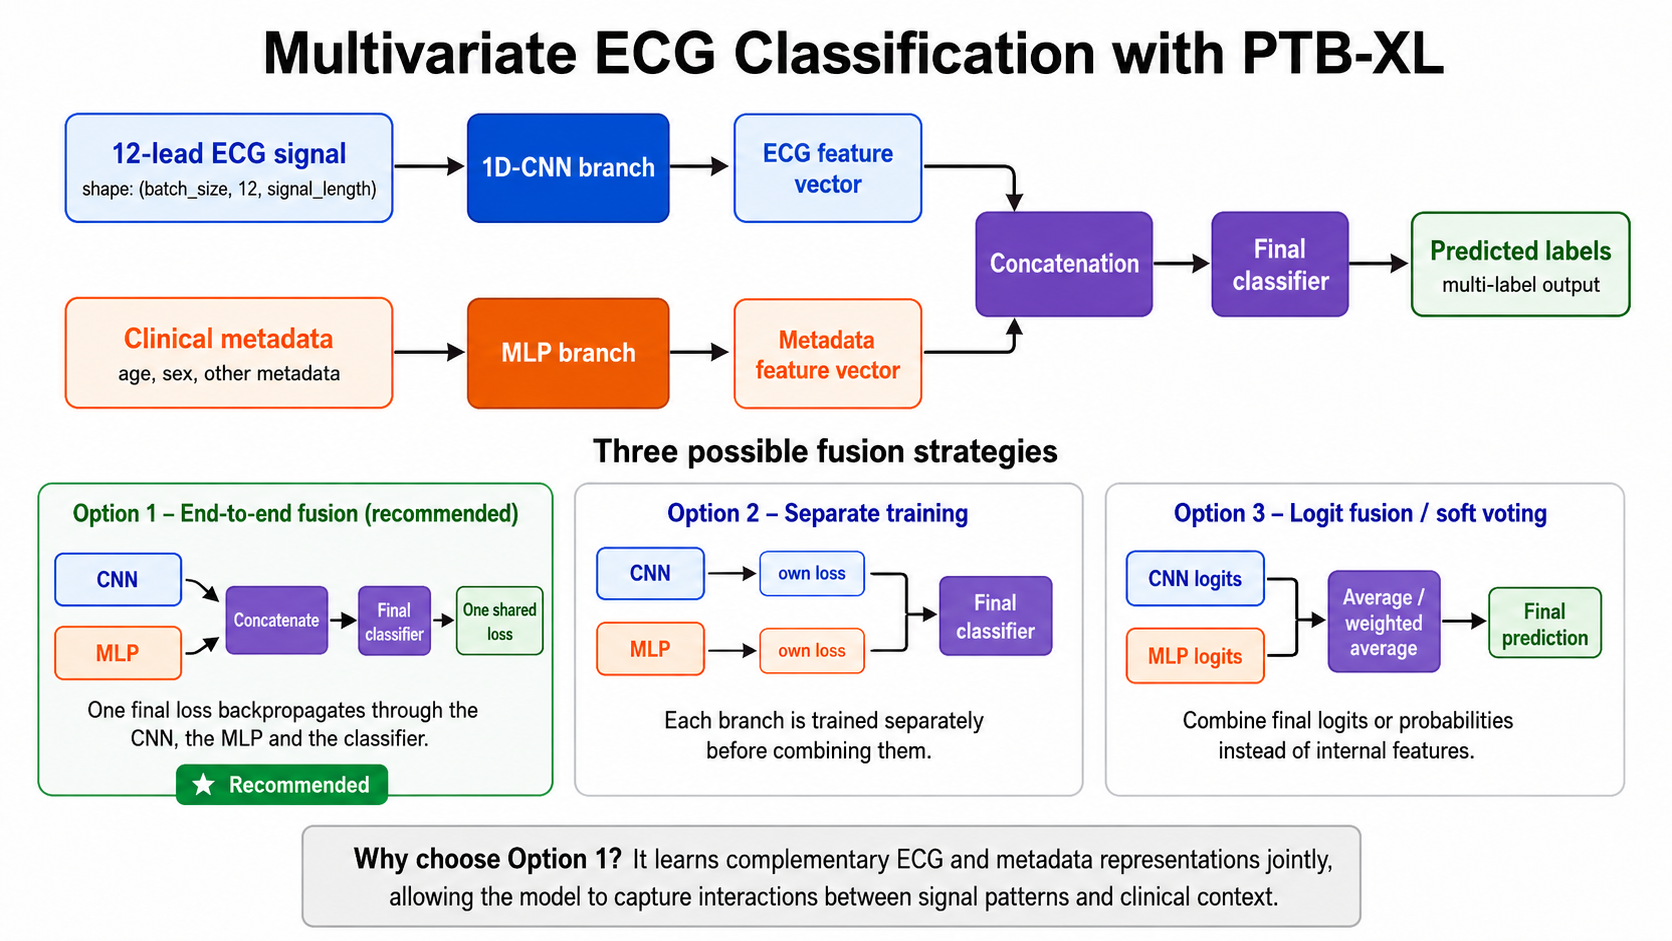
\includegraphics[width=0.98\textwidth]{figures/fusion_architecture.png}
    \caption{Overview of the multivariate PTB-XL architecture and the three possible fusion strategies considered during the project. The final selected model is Option 1: end-to-end feature-level fusion with one shared loss.}
    \label{fig:architecture}
\end{figure}

The ECG branch uses the following Conv1D progression:
\[
    12 \rightarrow 32 \rightarrow 64 \rightarrow 128 \rightarrow 128.
\]
The final adaptive average pooling produces a 128-dimensional ECG feature vector. The metadata MLP produces a 32-dimensional metadata feature vector. The classifier receives their concatenation:
\[
    z = [z_{ECG}; z_{meta}] \in \mathbb{R}^{160}.
\]
It then outputs five logits:
\[
    \hat{y} = f_{cls}(z) \in \mathbb{R}^{5}.
\]

The loss is computed as:
\[
\mathcal{L} = - \frac{1}{C}\sum_{c=1}^{C}\left[y_c \log(\sigma(\hat{y}_c)) + (1-y_c)\log(1-\sigma(\hat{y}_c))\right],
\]
where \(C=5\), and \(\sigma\) is the sigmoid function. In implementation, BCEWithLogitsLoss is used for numerical stability.

When backpropagation is applied to this single final loss, gradients update the ECG CNN, the metadata MLP and the final classifier at the same time. This was the main reason for choosing the shared-loss fusion model: the model can learn ECG morphology and clinical context jointly, instead of combining independent predictions only at the end.

\subsection{Alternative Fusion Strategies}

Three fusion strategies were considered:

\paragraph{Option 1: Shared-loss feature fusion.}
The ECG branch and metadata branch output internal feature representations. These are concatenated before the final classifier. A single loss updates all components jointly. This is the main model.

\paragraph{Option 2: Separate training.}
The ECG model and metadata model are trained separately, each with its own loss. Their features or outputs are later used by another classifier. This is easier to interpret but does not optimize both branches jointly.

\paragraph{Option 3: Logit fusion / soft voting.}
An ECG-only model and a metadata-only model are trained separately. Their final probabilities are combined by a weighted average:
\[
    p_{soft} = \alpha p_{ECG} + (1-\alpha)p_{meta}.
\]
This is used as a benchmark to test whether prediction-level fusion is competitive with shared-loss feature-level fusion.

\section{Implementation Evolution}

The implementation evolved through four versions. This section is included because it explains why the final code structure and training strategy changed during the project.

\begin{table}[H]
\centering
\caption{Evolution of the PTB-XL implementation.}
\begin{tabular}{p{1.8cm}p{12cm}}
\toprule
\textbf{Version} & \textbf{Main role} \\
\midrule
V1 & First modular PTB-XL pipeline. It introduced the main project structure, the dataset class, the CNN+MLP fusion model and a first training loop. It was mainly used to move away from notebooks and toward small Python files. \\
V2 & Debug version. It added progress prints and made it possible to understand whether the code was loading data, building dataloaders or training. A full fusion model trained successfully, but the PR-curve saving crashed because \code{np.trapz} was unavailable in the installed NumPy version. \\
V3 & Cache version. It fixed the PR-curve computation using \code{np.trapezoid} and added tensor caching so that ECG files were read only once. This made full PTB-XL training much faster and more reproducible. \\
V4 & Training-tools version. It added weight decay, a learning-rate scheduler, early stopping, threshold tuning on validation predictions, validation prediction saving and soft-voting support. This became the final experimental version. \\
\bottomrule
\end{tabular}
\label{tab:versions}
\end{table}

This progression was important because the initial full training was bottlenecked by repeated ECG file loading. The cache changed the workflow from reading thousands of WFDB files at every epoch to training directly from preprocessed tensors.

\section{Experimental Setup}

\subsection{Splits and Inputs}

The official PTB-XL fold split was used:
\begin{itemize}[noitemsep]
    \item folds 1--8 for training: 17,418 samples;
    \item fold 9 for validation: 2,183 samples;
    \item fold 10 for testing: 2,198 samples.
\end{itemize}
Each ECG tensor has shape \((12,1000)\). The metadata tensor has shape \((4)\), corresponding to age, sex, height and weight. Labels are five-dimensional multi-label targets.

\subsection{Training Configuration}

The main V4 fusion run used:
\begin{itemize}[noitemsep]
    \item 100 Hz ECG signals;
    \item batch size 64;
    \item Adam optimizer;
    \item learning rate 0.001;
    \item weight decay \(10^{-4}\);
    \item BCEWithLogitsLoss with positive class weights;
    \item early stopping with patience 6;
    \item ReduceLROnPlateau scheduler;
    \item validation-based threshold tuning.
\end{itemize}

The threshold tuning step was important because multi-label classification does not require the same probability threshold for every class. The tuned thresholds for the best fusion model were:
\[
    [0.65, 0.70, 0.50, 0.65, 0.60]
\]
for NORM, MI, STTC, CD and HYP respectively.

\subsection{Evaluation Metrics}

Because PTB-XL is multi-label and imbalanced, accuracy alone is not sufficient. The report uses:
\begin{itemize}[noitemsep]
    \item macro-precision, macro-recall and macro-F1;
    \item micro-precision, micro-recall and micro-F1;
    \item per-class F1-score;
    \item exact match accuracy;
    \item precision-recall curves.
\end{itemize}
Exact match accuracy is strict: a prediction is correct only if all five labels match exactly. Therefore, a moderate exact match score does not mean that the model is wrong on half of the labels; it means that the entire multi-label vector is perfectly correct for that proportion of ECG recordings.

\section{Results}

\subsection{MIT-BIH Baseline Results}

The MIT-BIH baseline reached strong results on the extracted heartbeat classification task. This is expected because the task is simpler than PTB-XL: each input is an isolated heartbeat window and the output is one class among five.

\begin{table}[H]
\centering
\caption{MIT-BIH baseline test results.}
\begin{tabular}{lrrrr}
\toprule
\textbf{Class} & \textbf{Precision} & \textbf{Recall} & \textbf{F1-score} & \textbf{Support} \\
\midrule
Normal & 0.9883 & 0.9790 & 0.9836 & 13592 \\
Supraventricular & 0.6591 & 0.6938 & 0.6760 & 418 \\
Ventricular & 0.9202 & 0.9659 & 0.9425 & 1086 \\
Fusion & 0.6265 & 0.8595 & 0.7247 & 121 \\
Unknown & 0.9885 & 0.9942 & 0.9913 & 1207 \\
\midrule
Macro average & 0.8365 & 0.8985 & 0.8636 & -- \\
Accuracy & \multicolumn{3}{c}{0.9711} & -- \\
\bottomrule
\end{tabular}
\label{tab:mitbih_results}
\end{table}

\begin{figure}[H]
    \centering
    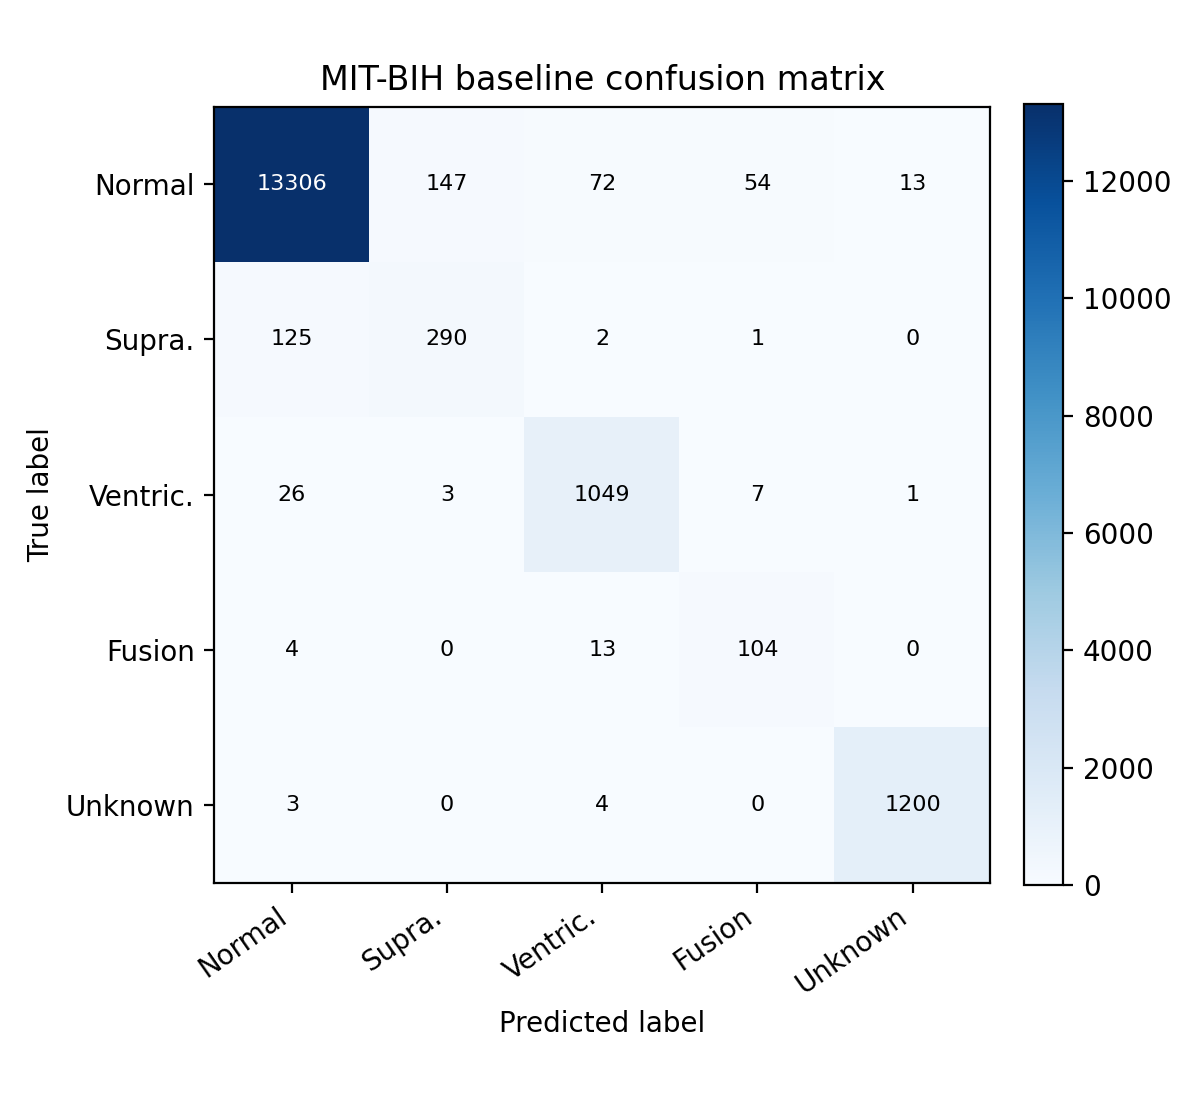
\includegraphics[width=0.72\textwidth]{figures/mitbih_confusion_matrix.png}
    \caption{Confusion matrix for the MIT-BIH heartbeat-level baseline. Errors mainly concern supraventricular and fusion beats, while normal and unknown beats are classified very well.}
    \label{fig:mitbih_cm}
\end{figure}

The baseline confirms that a 1D-CNN can learn useful local ECG morphology. However, the high accuracy should not be overinterpreted for the final project because this task is easier and less clinically contextual than PTB-XL.

\subsection{PTB-XL Model Comparison}

The final PTB-XL experiments compare four approaches:
\begin{enumerate}[noitemsep]
    \item metadata-only MLP;
    \item ECG-only CNN;
    \item soft voting between ECG-only and metadata-only predictions;
    \item shared-loss fusion CNN+MLP.
\end{enumerate}

\begin{table}[H]
\centering
\caption{Main PTB-XL test metrics for all final models.}
\begin{tabular}{lrrrr}
\toprule
\textbf{Model} & \textbf{Macro-F1} & \textbf{Micro-F1} & \textbf{Exact match} & \textbf{Test loss} \\
\midrule
Metadata-only MLP & 0.4645 & 0.4909 & 0.2234 & 0.9446 \\
ECG-only CNN & 0.7091 & 0.7497 & 0.5528 & 0.6156 \\
Soft voting & 0.7084 & 0.7491 & 0.5523 & -- \\
Shared-loss fusion & \textbf{0.7108} & \textbf{0.7536} & \textbf{0.5660} & \textbf{0.5928} \\
\bottomrule
\end{tabular}
\label{tab:model_comparison}
\end{table}

\begin{figure}[H]
    \centering
    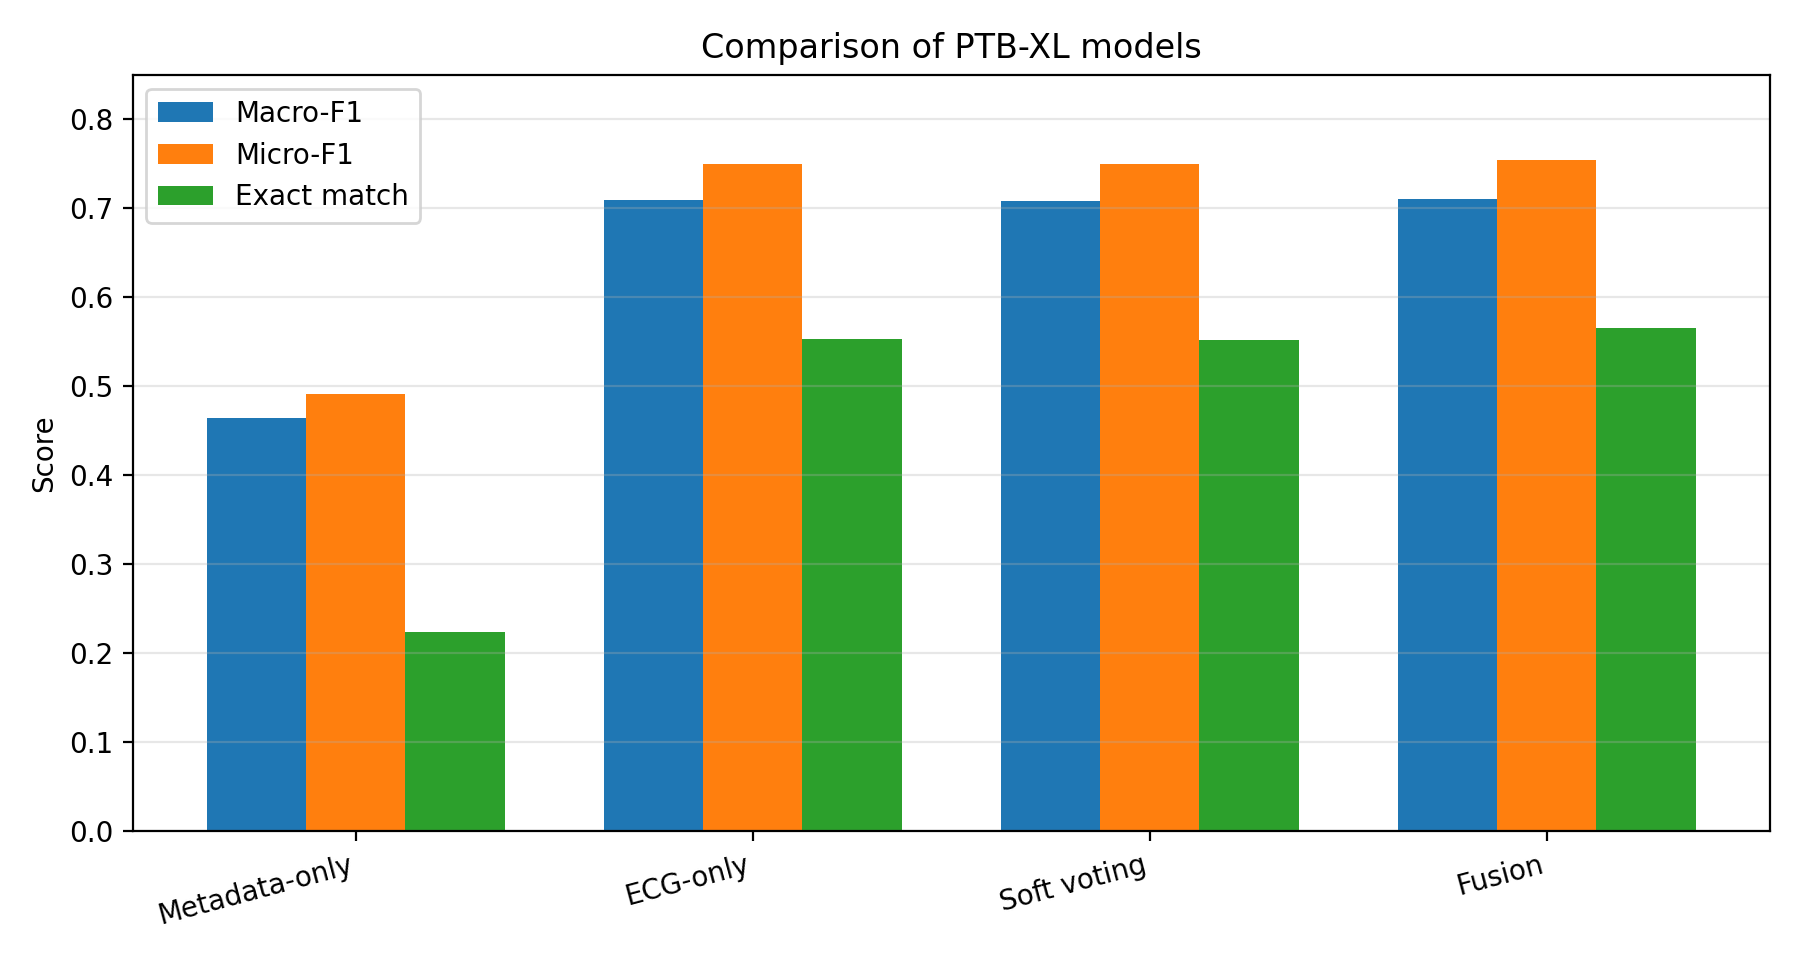
\includegraphics[width=0.9\textwidth]{figures/model_comparison_metrics.png}
    \caption{Comparison of the main PTB-XL models. The fusion model performs best overall, although the improvement over ECG-only is modest.}
    \label{fig:model_comparison}
\end{figure}

The metadata-only model performs much worse than models using ECG signals. This shows that age, sex, height and weight alone are not sufficient to solve the diagnostic classification problem. However, the shared-loss fusion model slightly improves over ECG-only. This suggests that metadata can provide complementary context, but the ECG signal remains the dominant source of information.

\subsection{Per-Class Results}

\begin{table}[H]
\centering
\caption{Per-class F1-scores on the PTB-XL test set.}
\begin{tabular}{lrrrrr}
\toprule
\textbf{Model} & \textbf{NORM} & \textbf{MI} & \textbf{STTC} & \textbf{CD} & \textbf{HYP} \\
\midrule
Metadata-only & 0.6984 & 0.4920 & 0.4521 & 0.4018 & 0.2783 \\
ECG-only & 0.8520 & 0.7395 & \textbf{0.7628} & \textbf{0.7343} & 0.4569 \\
Soft voting & 0.8520 & 0.7391 & 0.7623 & 0.7347 & 0.4540 \\
Shared-loss fusion & \textbf{0.8556} & \textbf{0.7480} & 0.7493 & 0.7251 & \textbf{0.4757} \\
\bottomrule
\end{tabular}
\label{tab:per_class_f1}
\end{table}

\begin{figure}[H]
    \centering
    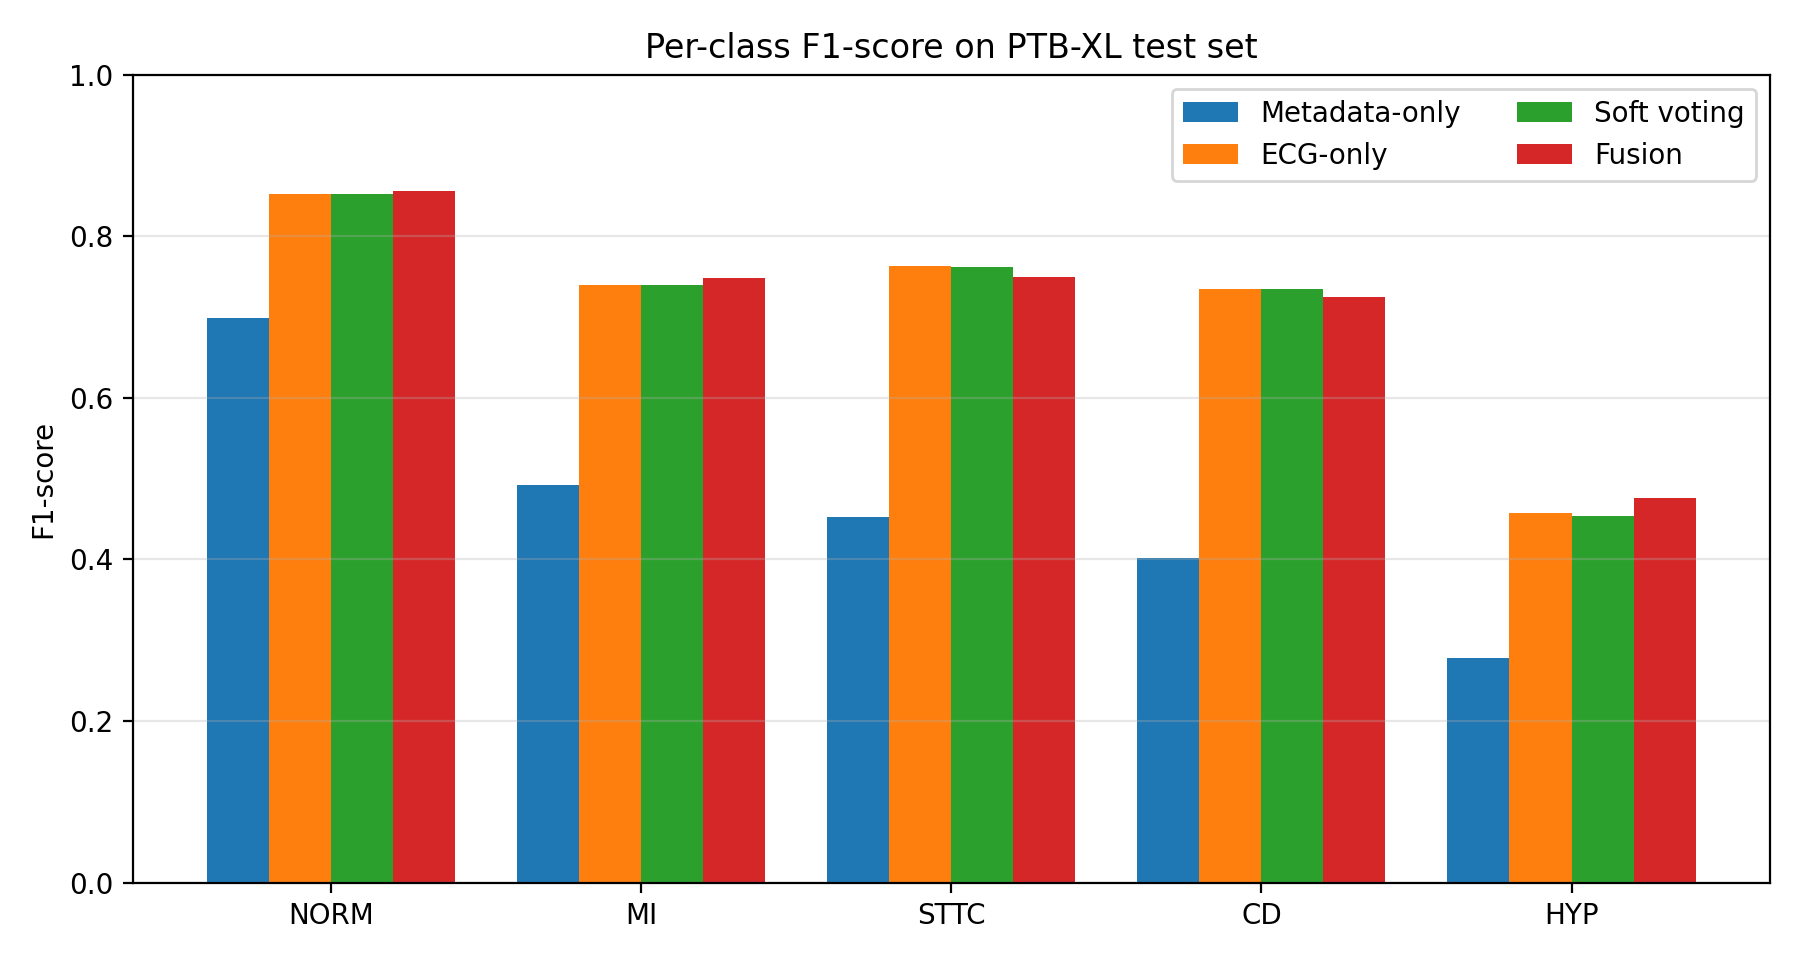
\includegraphics[width=0.9\textwidth]{figures/per_class_f1_comparison.png}
    \caption{Per-class F1-score comparison. HYP is the weakest class for all models, which is consistent with the imbalance and diagnostic difficulty reported in related work.}
    \label{fig:per_class_f1}
\end{figure}

The shared-loss fusion model improves NORM, MI and HYP compared with ECG-only, but ECG-only remains slightly better on STTC and CD. Therefore, the fusion model should be interpreted as a modest improvement, not as a dramatic breakthrough. This is still valuable: it shows that feature-level fusion can extract some useful information from metadata, but the signal itself carries most of the predictive power.

\subsection{Training and Precision-Recall Curves}

\begin{figure}[H]
    \centering
    \begin{subfigure}{0.49\textwidth}
        \centering
        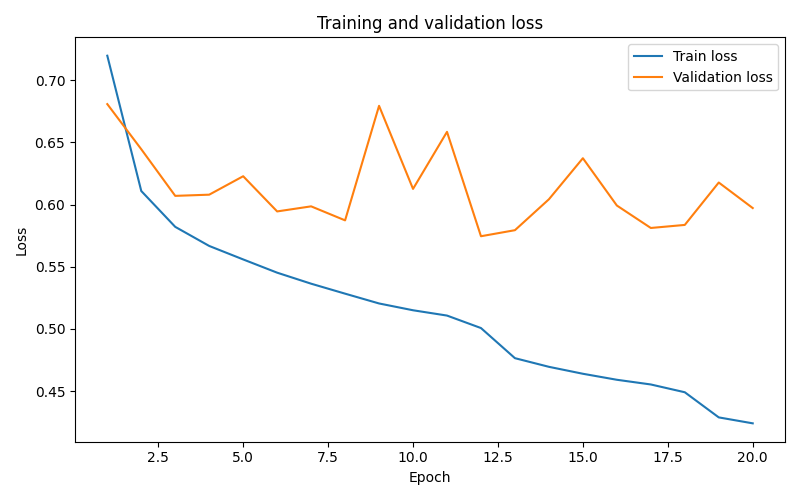
\includegraphics[width=\textwidth]{figures/fusion_training_curves.png}
        \caption{Loss curves}
    \end{subfigure}
    \begin{subfigure}{0.49\textwidth}
        \centering
        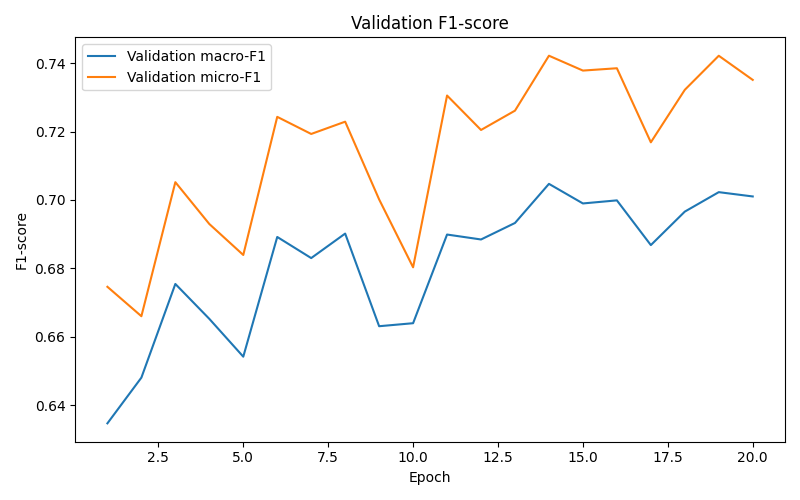
\includegraphics[width=\textwidth]{figures/fusion_validation_f1_curves.png}
        \caption{Validation F1 curves}
    \end{subfigure}
    \caption{Training dynamics of the final fusion model. The scheduler reduced the learning rate during training, and early stopping selected the best checkpoint according to validation macro-F1.}
    \label{fig:fusion_training}
\end{figure}

\begin{figure}[H]
    \centering
    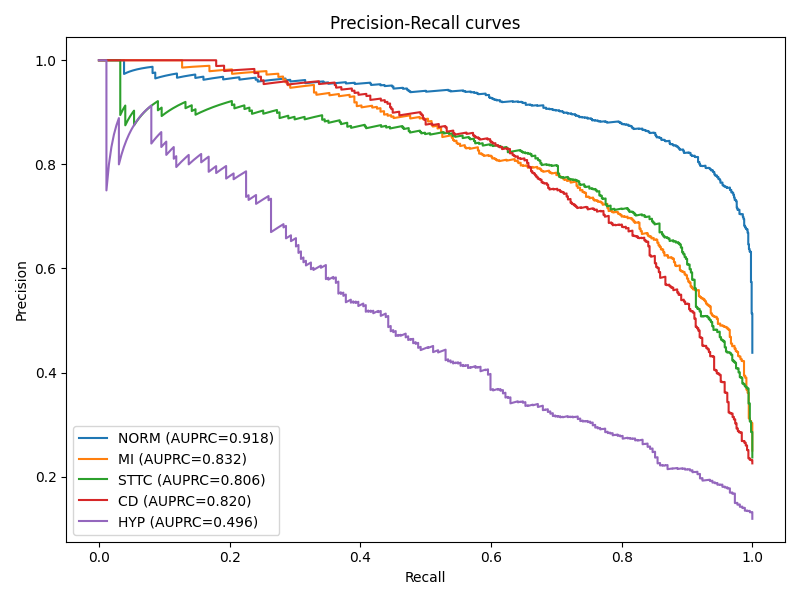
\includegraphics[width=0.82\textwidth]{figures/fusion_pr_curves.png}
    \caption{Precision-recall curves for the final shared-loss fusion model. These curves are more informative than a single accuracy value because PTB-XL is multi-label and imbalanced.}
    \label{fig:fusion_pr}
\end{figure}

The final fusion run reached its best validation macro-F1 before threshold tuning at epoch 14. Threshold tuning improved validation macro-F1 to 0.7193 and produced the final class thresholds used on the test set. This step improved the precision-recall balance compared with a fixed threshold of 0.5.

\subsection{Soft Voting Benchmark}

Soft voting was implemented as a prediction-level fusion benchmark. The validation search selected:
\[
    \alpha = 0.9.
\]
This means that the best soft-voting ensemble relied 90\% on the ECG-only model and only 10\% on the metadata-only model. This confirms that metadata-only predictions are weak and that the ECG signal is the main source of useful information.

The soft-voting test macro-F1 was 0.7084, slightly below the shared-loss fusion macro-F1 of 0.7108. This supports the choice of shared-loss fusion: learning a joint representation before the classifier is slightly more effective than averaging final predictions.

\section{Discussion}

\subsection{Was Metadata Useful?}

The answer is yes, but only modestly. The metadata-only model is clearly insufficient, with macro-F1 0.4645. This means that age, sex, height and weight cannot replace ECG morphology. However, when metadata is fused with ECG features through the shared-loss model, performance improves slightly over ECG-only and soft voting.

This suggests that metadata provides weak but complementary context. The improvement is not large, so the report should avoid overclaiming. A careful conclusion is that the metadata branch helps a little, but the 12-lead ECG remains the core input.

\subsection{Why Shared-Loss Fusion?}

The shared-loss fusion model is justified by both architecture and results. Architecturally, it is more integrated than soft voting: it combines learned ECG and metadata representations before classification. Experimentally, it obtains the best macro-F1, micro-F1, exact match accuracy and test loss among the final models.

However, the difference between ECG-only and fusion is small. This is also informative: the 12-lead ECG already contains the most discriminative information, and simple metadata cannot fundamentally change the classification difficulty.

\subsection{Main Limitation: HYP}

HYP remains the weakest class across all models. In the final fusion model, HYP F1 is 0.4757. Related PTB-XL work also reports HYP as difficult, with weaker performance than the other classes \cite{mehdi2026ptbxl}. This may be due to class imbalance, subtle ECG manifestations, label uncertainty, or overlap with other diagnostic patterns.

Possible improvements include focal loss, more aggressive class balancing, oversampling, lead-wise normalization, longer training with early stopping, or architecture changes such as residual blocks or attention mechanisms.

\subsection{Comparison with the Reference Study}

The reference CNN-VAE study reports stronger weighted F1 and AUC values, but it uses a different architecture and stronger data-centric preprocessing, including class balancing and longer training \cite{mehdi2026ptbxl}. Our model is simpler and focuses on multimodal fusion rather than VAE-based representation learning. Therefore, the comparison should be treated as contextual, not direct.

Still, our results are in a reasonable range for a first modular PTB-XL fusion pipeline. The most important contribution of this project is not achieving state-of-the-art performance, but building a complete and explainable pipeline: raw PTB-XL loading, tensor caching, 12-lead CNN modeling, metadata fusion, threshold tuning, soft-voting comparison, and precision-recall evaluation.

\section{Limitations and Future Work}

The main limitations are:
\begin{itemize}[noitemsep]
    \item only four metadata variables were used;
    \item no advanced resampling strategy was applied;
    \item thresholds were tuned, but the architecture was not extensively optimized;
    \item HYP remains weak;
    \item no external dataset was used for generalization testing;
    \item no interpretability method was applied to identify which ECG leads or time regions influenced predictions.
\end{itemize}

Future work could include:
\begin{itemize}[noitemsep]
    \item lead-wise normalization based on training statistics;
    \item focal loss or improved class weighting;
    \item oversampling or balanced batch sampling for minority classes;
    \item residual 1D-CNN blocks;
    \item attention mechanisms over leads or time windows;
    \item calibration analysis and class-specific operating thresholds;
    \item interpretability methods such as saliency maps or SHAP explanations.
\end{itemize}

\section{Conclusion}

This project evolved from a simple MIT-BIH heartbeat-level baseline to a modular PTB-XL multivariate ECG classification pipeline. The MIT-BIH baseline validated the basic 1D-CNN workflow. The PTB-XL extension introduced 12-lead ECG signals, static clinical metadata and multi-label classification over five diagnostic superclasses.

The final shared-loss fusion model combines a 1D-CNN ECG branch with an MLP metadata branch. It outperforms metadata-only, ECG-only and soft-voting baselines, although the improvement over ECG-only is modest. This supports the conclusion that metadata provides complementary clinical context, but that the ECG signal remains the dominant predictive source.

The final model reaches a test macro-F1 of 0.7108 and a micro-F1 of 0.7536. The strongest classes are NORM, MI, STTC and CD, while HYP remains the main weakness. Overall, the project provides a clean, reproducible and well-structured foundation for multivariate ECG classification and leaves clear directions for further improvement.

\appendix
\newpage
\section{Additional Figures}

\begin{figure}[H]
    \centering
    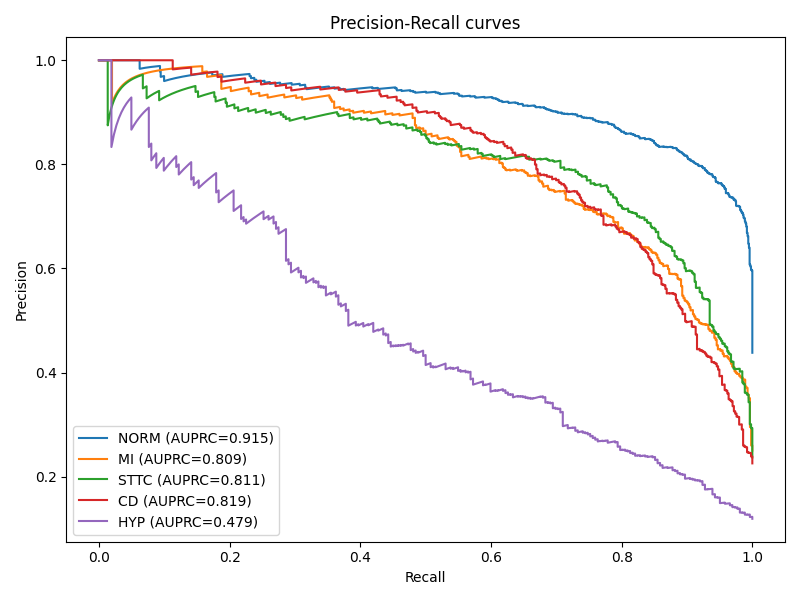
\includegraphics[width=0.82\textwidth]{figures/ecg_only_pr_curves.png}
    \caption{Precision-recall curves for the ECG-only V4 model.}
\end{figure}

\begin{figure}[H]
    \centering
    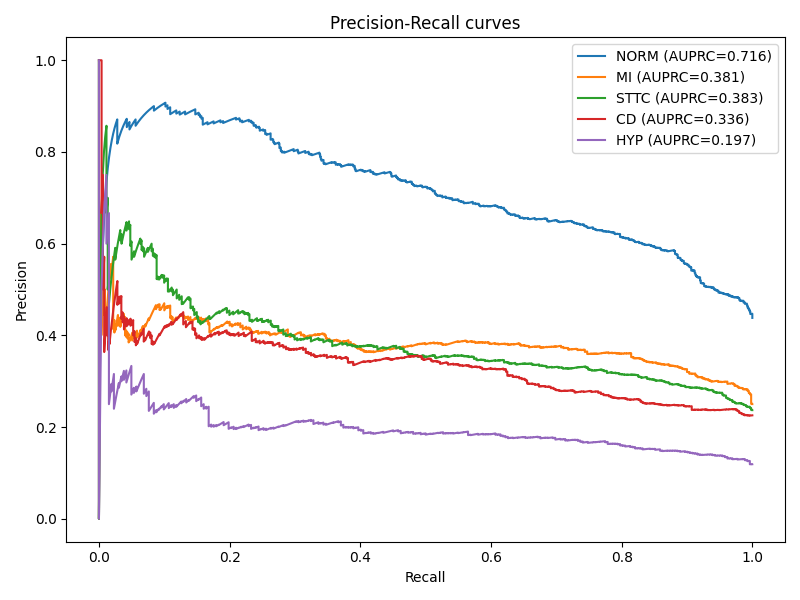
\includegraphics[width=0.82\textwidth]{figures/metadata_only_pr_curves.png}
    \caption{Precision-recall curves for the metadata-only model. The weak performance confirms that static metadata alone is insufficient.}
\end{figure}

\begin{figure}[H]
    \centering
    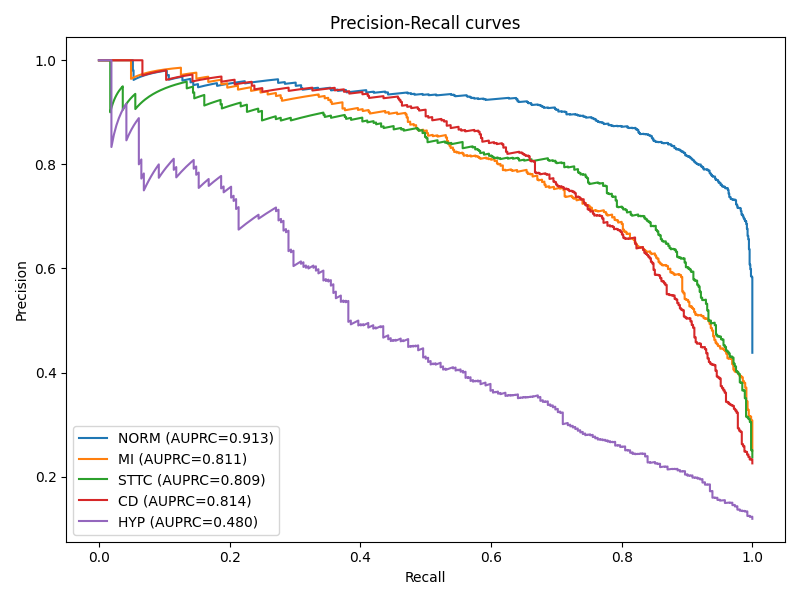
\includegraphics[width=0.82\textwidth]{figures/soft_voting_pr_curves.png}
    \caption{Precision-recall curves for the soft-voting benchmark.}
\end{figure}

\section{Run Summary}

The final analysis is based on four main experiment folders:

\begin{itemize}
    \item \code{20260521\_154229\_fusion}: final V4 shared-loss fusion run with scheduler, early stopping, threshold tuning and full PTB-XL split.
    \item \code{20260521\_160125\_ecg\_only}: final V4 ECG-only benchmark using only the 12-lead ECG signal and threshold tuning.
    \item \code{20260521\_154953\_metadata\_only}: metadata-only MLP benchmark using age, sex, height and weight.
    \item \code{20260521\_160422\_soft\_voting}: soft-voting benchmark combining ECG-only and metadata-only predictions.
\end{itemize}

\newpage
\begin{thebibliography}{9}

\bibitem{wagner2020ptbxl}
P. Wagner, N. Strodthoff, R.-D. Bousseljot, D. Kreiseler, F. I. Lunze, W. Samek, and T. Schaeffter.
\newblock PTB-XL, a large publicly available electrocardiography dataset.
\newblock \emph{Scientific Data}, 7(154), 2020.

\bibitem{goldberger2000physiobank}
A. L. Goldberger, L. A. N. Amaral, L. Glass, J. M. Hausdorff, P. Ch. Ivanov, R. G. Mark, J. E. Mietus, G. B. Moody, C.-K. Peng, and H. E. Stanley.
\newblock PhysioBank, PhysioToolkit, and PhysioNet: Components of a new research resource for complex physiologic signals.
\newblock \emph{Circulation}, 101(23):e215--e220, 2000.

\bibitem{moody2001mitdb}
G. B. Moody and R. G. Mark.
\newblock The impact of the MIT-BIH Arrhythmia Database.
\newblock \emph{IEEE Engineering in Medicine and Biology Magazine}, 20(3):45--50, 2001.

\bibitem{mehdi2026ptbxl}
N. A. Mehdi and A. A. Drigh.
\newblock ECG Classification on PTB-XL: A Data-Centric Approach with Simplified CNN-VAE.
\newblock \emph{arXiv preprint arXiv:2603.07558}, 2026.

\bibitem{ribeiro2020automatic}
A. H. Ribeiro, M. H. Ribeiro, G. M. M. Paixao, D. M. Oliveira, P. R. Gomes, J. A. Canazart, M. P. S. Ferreira, C. R. Andersson, P. W. Macfarlane, W. Meira Jr., and others.
\newblock Automatic diagnosis of the 12-lead ECG using a deep neural network.
\newblock \emph{Nature Communications}, 11:1760, 2020.

\end{thebibliography}

\end{document}
